\documentclass[10pt]{exam}
\usepackage[phy]{template-for-exam}
\usepackage{tikz}
\usetikzlibrary{decorations.pathmorphing,patterns}
\header{Name:}{Date:}{Period: \hspace{2cm} ID:A}


\title{Projectile Motion - Quiz I}
\author{Rohrbach}
\date{\today}

\begin{document}
\maketitle

\noindent
A child runs straight off a high-dive platform with a horizontal velocity of 1.1 m/s.  He lands in the water, 4.2 meters below

\vspace{2em}


\begin{parts}
  \part
    Label this diagram of the situation and {\bf make a T-chart} to list your knowns and unknowns. (3 points)
  
    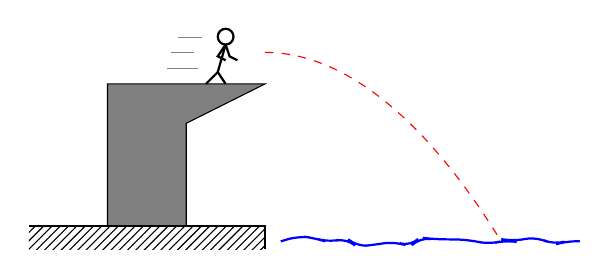
\begin{tikzpicture}
      \draw[
        thick,
        blue,
        rounded corners,
        decorate,
        decoration={
          random steps,
          segment length=2mm,
          amplitude=2pt
          }] (3.2,0) -- (7,0);
    \draw[fill=gray] (2,.2)
        -- ++(0,1.3)
        -- ++(1,.5)
        -- ++(-2,0)
        -- ++(0,-1.8)
        -- cycle;
      \fill[white,pattern color=black, pattern= north east lines] (0,-.1) rectangle (3,.2);
      \draw[thick] (0,.2) -| (3,-.1);
      \draw[dashed,red] (3,2.4) parabola (6,0);

      \begin{scope}[shift={(2.5,2)},scale=0.5,thick]
        \draw (0,1.2) circle (0.2);
        \coordinate (waste) at (-.2,.3);
        \coordinate (neck) at (0,1);
        \draw (waste) -- (neck);
        \draw (-.5,0) -- (waste);
        \draw (0,0) -- (waste);
        \draw (neck) -- ++(.1,-.3) -- ++(.2,-.1);
        \draw (neck) -- ++(-.2,-.3) -- ++(.2,-.1);
      \end{scope}

        \draw[ultra thin, gray] (2.2,2.6) -- ++(-.3,0);
        \draw[ultra thin, gray] (2.1,2.4) -- ++(-.3,0);
        \draw[ultra thin, gray] (2.15,2.2) -- ++(-.4,0);


    \end{tikzpicture}

  \part
    How long will it take the child to reach the water? (3 points)
    \vs
  
  \part
    What horizontal distance will the child move before hitting the water? (3 points)
    \vs
  
  \part
    What are the $x$- and $y$- components of the child's velocity just before he hits the water? (3 points)
    \vs
  
  \part
    Draw a triangle and calculate the magnitude and direction of the child’s resultant velocity just before hitting the water. (3 points)
    \vs

    
\end{parts}


\end{document}